\hypertarget{index_intro_sec}{}\section{Introduction}\label{index_intro_sec}
The {\bfseries A\+Log} data logger is an Arduino-\/based data logger that includes a full software library and documentation. The goal of this documentation is to ease the transition of researchers from closed-\/source proprietary technologies that are often well-\/documented, but can be expensive black boxes, to a fully open-\/source hardware and software toolchain that gives researchers all the power to control their data collection. For citizen-\/scientists who are interested in this tool\+: welcome, and it is greatly hoped that these instructions will suffice to get you started on the road to making measurements of our natural environment.\hypertarget{index_software}{}\section{Software Installation}\label{index_software}
All of our software is available from our Git\+Hub repository, \href{https://github.com/NorthernWidget}{\tt https\+://github.\+com/\+Northern\+Widget}. To install the Arduino software and the core libraries, follow these steps\+:\hypertarget{index_libraries}{}\subsection{A\+Log program and libraries}\label{index_libraries}

\begin{DoxyEnumerate}
\item Download Arduino’s latest I\+DE (version 1.\+6.\+9 at the time of writing)\+: \href{http://arduino.cc/en/Main/Software}{\tt http\+://arduino.\+cc/en/\+Main/\+Software}
\item Navgate to your {\bfseries sketchbook} folder in your home directory, and into the {\bfseries libraries} folder that it contains. Clone or download the following git repositories there\+:
\end{DoxyEnumerate}
\begin{DoxyEnumerate}
\item 1. The main \hyperlink{classLogger}{Logger} library\+: \href{https://github.com/NorthernWidget/Logger}{\tt https\+://github.\+com/\+Northern\+Widget/\+Logger}
\end{DoxyEnumerate}
\begin{DoxyEnumerate}
\item 2. The D\+S3231 clock library\+: \href{https://github.com/NorthernWidget/DS3231}{\tt https\+://github.\+com/\+Northern\+Widget/\+D\+S3231}.
\end{DoxyEnumerate}
\begin{DoxyEnumerate}
\item 3. Sd\+Fat library\+: \href{https://github.com/greiman/SdFat}{\tt https\+://github.\+com/greiman/\+Sd\+Fat}
\item In order to communicate with the A\+Log outside of the Arduino I\+DE (step 1) and set its clock, you will want to download A\+Log\+Talk from our Git\+Hub repository, \href{https://github.com/NorthernWidget/ALogTalk,}{\tt https\+://github.\+com/\+Northern\+Widget/\+A\+Log\+Talk,} along with Python if you are running Windows (Linux and Mac users have Python by default). See \href{http://www.python.org/getit/}{\tt http\+://www.\+python.\+org/getit/}.
\end{DoxyEnumerate}

Once all of these are installed, you are ready to program your A\+Log. Our Quick Start Guide is in the works, and will provide the next steps. Please e-\/mail \href{mailto:info@northernwidget.com}{\tt info@northernwidget.\+com} (for the full team) or Chad Sandell (\href{mailto:sand0724@umn.edu}{\tt sand0724@umn.\+edu}) if you have questions\hypertarget{index_arduino_tutorial}{}\subsection{Arduino}\label{index_arduino_tutorial}
Limor Fried has an excellent tutorial for Arduino at \href{http://www.ladyada.net/learn/arduino/}{\tt http\+://www.\+ladyada.\+net/learn/arduino/}. If you are unfamiliar with the platform (and/or embedded electronics), I strongly suggest that you purchase and Arduino Uno (\href{http://arduino.cc/en/Main/arduinoBoardUno}{\tt http\+://arduino.\+cc/en/\+Main/arduino\+Board\+Uno}), which is their basic board upon which the A\+Log Bottle\+Logger is based, and run through these tutorials to get used to C/\+C++ programming and Arduino.\hypertarget{index_quickstart}{}\section{Quick-\/start guide}\label{index_quickstart}
{\itshape This section, our quick-\/start guide is meant to get you up and running with your A\+Log Bottle\+Logger as efficiently as possible.}

All right. You have your A\+Log data logger, and you’re ready to measure... something. Anything, really. But you need a hand getting out of the blocks. This section is here for you.\hypertarget{index_software_install}{}\subsection{Installing requisite software}\label{index_software_install}
Go to \hyperlink{index_libraries}{A\+Log program and libraries}, above, and follow the installation directions.\hypertarget{index_program_upload}{}\subsection{Upload the program \char`\"{}alog\+\_\+no\+\_\+sensors\char`\"{}}\label{index_program_upload}
Now, upload some code to your data logger. We’ll start with an example that does nothing but log the time. Follow these steps\+:


\begin{DoxyEnumerate}
\item Start the Arduino application on your computer.
\item Go to File→\+Examples→\+Logger→alog\+\_\+no\+\_\+sensors. Click to open it.  
\begin{DoxyImage}
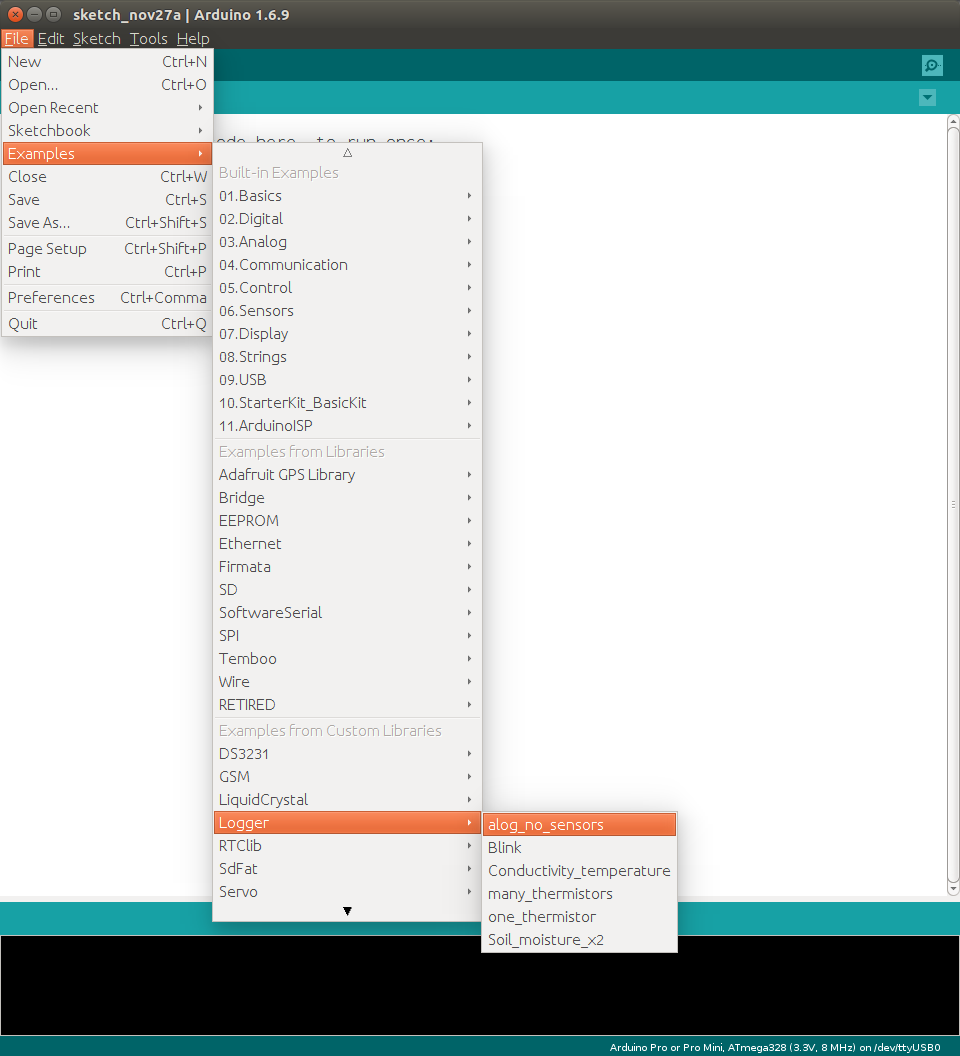
\includegraphics[width=.8\linewidth]{Open_alog_no_sensors.png}
\caption{Open alog\+\_\+no\+\_\+sensors\+: this is our blank template upon which you can write your logger code. For now, we will just upload this file alone.}
\end{DoxyImage}

\item Select \char`\"{}\+Arduino Pro\char`\"{} under \char`\"{}boards\char`\"{}. Sparkfun’s Arduino Pro 3.\+3V has the same microcontroller chip and clock speed as the A\+Log Bottle\+Logger, so its settings are compatible.  
\begin{DoxyImage}
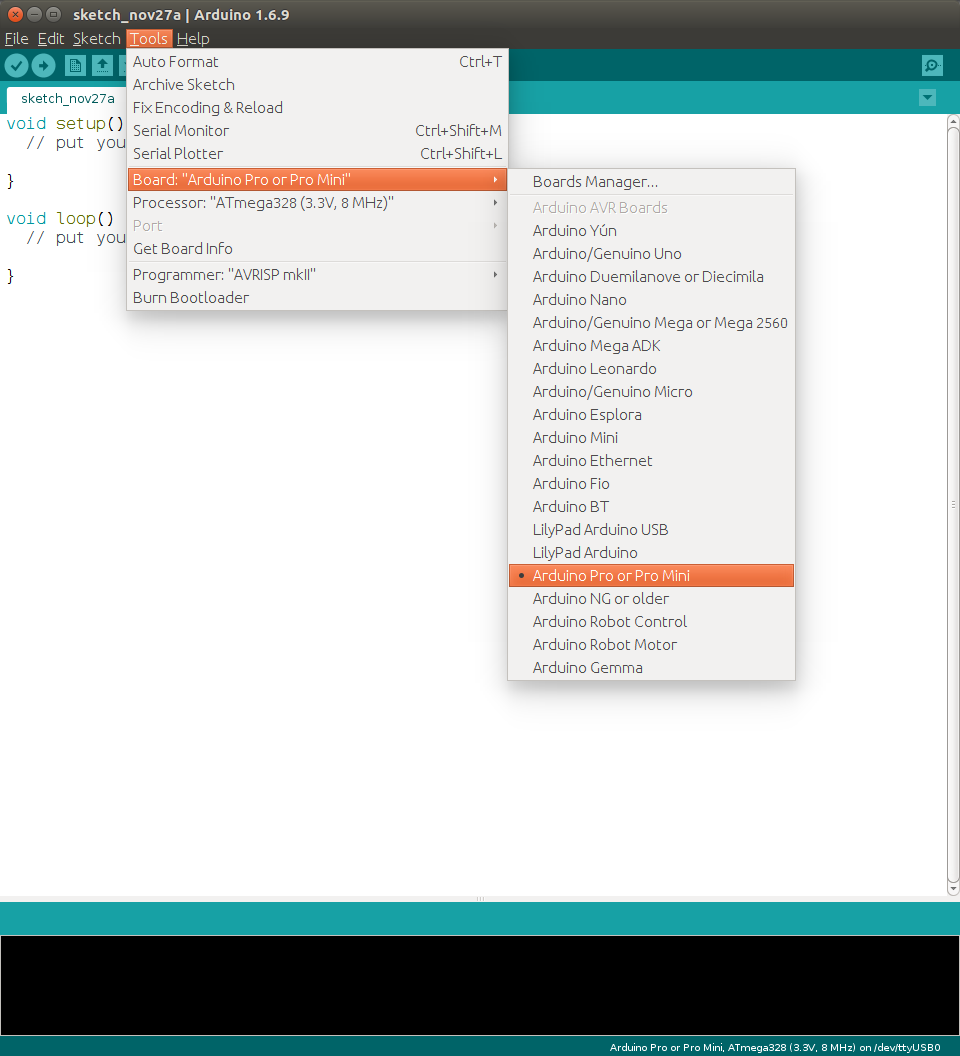
\includegraphics[width=.8\linewidth]{BoardsSelect_ArduinoPro.png}
\caption{Sparkfun\textquotesingle{}s Arduino pro can have the same settings as the A\+Log.}
\end{DoxyImage}

\item Select the processor for the A\+Log\+: 8 M\+Hz Arduino Pro 328.  
\begin{DoxyImage}
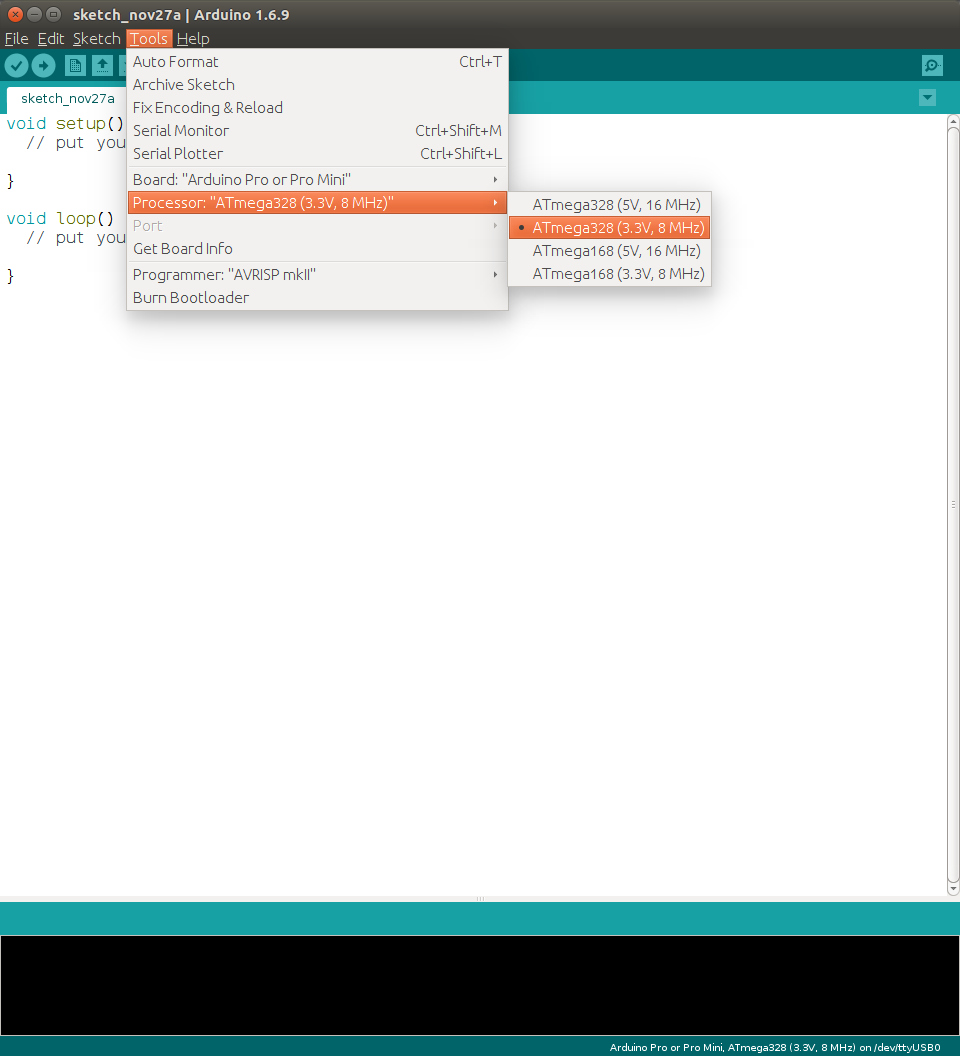
\includegraphics[width=.8\linewidth]{ProcessorSelect_3V3_8MHz.png}
\caption{The Arduino Pro or Pro Mini (3.3V, 8 M\+Hz) w/ A\+Tmega328 has the proper settings for the A\+Log Bottle\+Logger. Your version of Arduino won’t have the \textquotesingle{}A\+Log Bottle\+Logger\textquotesingle{} custom setting at the top; it is part of our work to eventually have a more streamlined A\+Log programming interface.}
\end{DoxyImage}

\item Plug in your A\+Log Bottle\+Logger using a U\+SB A to B cable.
\item The Bottle\+Logger should blink a couple of times on the L\+E\+D’s that are right by the U\+SB port. This means that it sees that it has been plugged in. Sometimes, we ship the Bottle\+Loggers with a \char`\"{}blink\char`\"{} program installed. This will cause the large red L\+ED in the center to blink when the A\+Log is plugged in... so your board might do this too. It’s one of our ways of testing that the board is programmable before shipping it to you.
\item Click on the \char`\"{}tools\char`\"{} menu, like the above figure. The \char`\"{}\+Serial Port\char`\"{} item in that menu should no longer be grayed out. Select your serial port.
\item Click \char`\"{}upload\char`\"{} from within the window holding \char`\"{}alog\+\_\+no\+\_\+sensors\char`\"{}, and send the code to the A\+Log. It will compile for a little while first, and then be sent over as a bitstream while the two small L\+E\+D’s by the U\+SB port on the A\+Log blink furiously\+: these are telling you that data is being sent to the logger (RX) or transmitted from the logger to the computer (TX).
\item Once this is done, click the \char`\"{}\+Serial Monitor\char`\"{} button to see what your data logger says. It will probably say something about setting the clock while the A\+Log flashes a syncopated rhythm on its main L\+ED. This means that it is time for your next step...
\end{DoxyEnumerate}\hypertarget{index_clock_setting}{}\subsection{Interfacing with the A\+Log and setting its clock}\label{index_clock_setting}
To set the clock of the A\+Log, plug it into your computer and run the \char`\"{}\+A\+Log\+Talk.\+py\char`\"{} program. This requires a Python interpreter (standard on all Linux and Mac computers) and can be done from the terminal by navigating to the A\+Log\+Talk directory and doing one of two things.

First, if you have a standard

F\+I\+N\+I\+SH T\+H\+IS A\+F\+T\+ER W\+O\+R\+K\+I\+NG T\+H\+R\+O\+U\+GH C\+L\+O\+CK S\+E\+T\+T\+I\+NG P\+R\+O\+G\+R\+A\+M\+S! S\+EE IF Y\+OU C\+AN G\+ET T\+HE H\+A\+N\+D\+S\+H\+A\+KE TO W\+O\+R\+K!

\begin{quote}
\begin{quote}
\begin{quote}
python A\+Log\+Talk.\+py \end{quote}
\end{quote}
\end{quote}


Instructions will appear on the screen; if the logger does not respond, you can push its \char`\"{}reset\char`\"{} button.

\begin{quote}
\begin{quote}
\begin{quote}
python A\+Log\+Talk.\+py \end{quote}
\end{quote}
\end{quote}


Instructions will appear on the screen; if the logger does not respond, you can push its \char`\"{}reset\char`\"{} button.\hypertarget{index_programming_your_own}{}\subsection{Creating and uploading a custom data logging routine}\label{index_programming_your_own}
The Github repository has examples of data logging routines, which you can modify for your own purposes. See the \char`\"{}examples\char`\"{} folder. You can also look at \char`\"{}\+Logger.\+h\char`\"{} to see what variables you need to pass to each sensor’s function.

These examples include comments for where you should place your commands to communicate with various sensors, both analog and digital.

If you are unfamiliar with C or Arduino programming, the Arduino reference guide can help\+: \href{http://arduino.cc/en/Reference/HomePage}{\tt http\+://arduino.\+cc/en/\+Reference/\+Home\+Page}.

{\bfseries I\+M\+P\+O\+R\+T\+A\+NT\+:} many examples of A\+Log code are included in this package; please use them as possible starting points for your code.\hypertarget{index_attaching_sensors}{}\subsection{Attaching sensors}\label{index_attaching_sensors}
Use the screw terminals (labeled) to connect sensors to the logger. These screw terminals are labeled with pin numbers that correspond to the pin numbers used in the program.\hypertarget{index_self_made_sensor_code}{}\subsection{Writing your own sensor code}\label{index_self_made_sensor_code}
\hypertarget{index_field_deployment}{}\subsection{Field deployment}\label{index_field_deployment}
We have learned a bit from past field installations, so you can e-\/mail us at \href{mailto:info@northernwidget.com}{\tt info@northernwidget.\+com} to tell us that you want some of these examples on the website. In the meantime, it’s basically an exercise in keeping the logger away from the elements and animals that like to chew wires.\hypertarget{index_pinout}{}\section{A\+Log pinout and peripherals}\label{index_pinout}
 
\begin{DoxyImage}
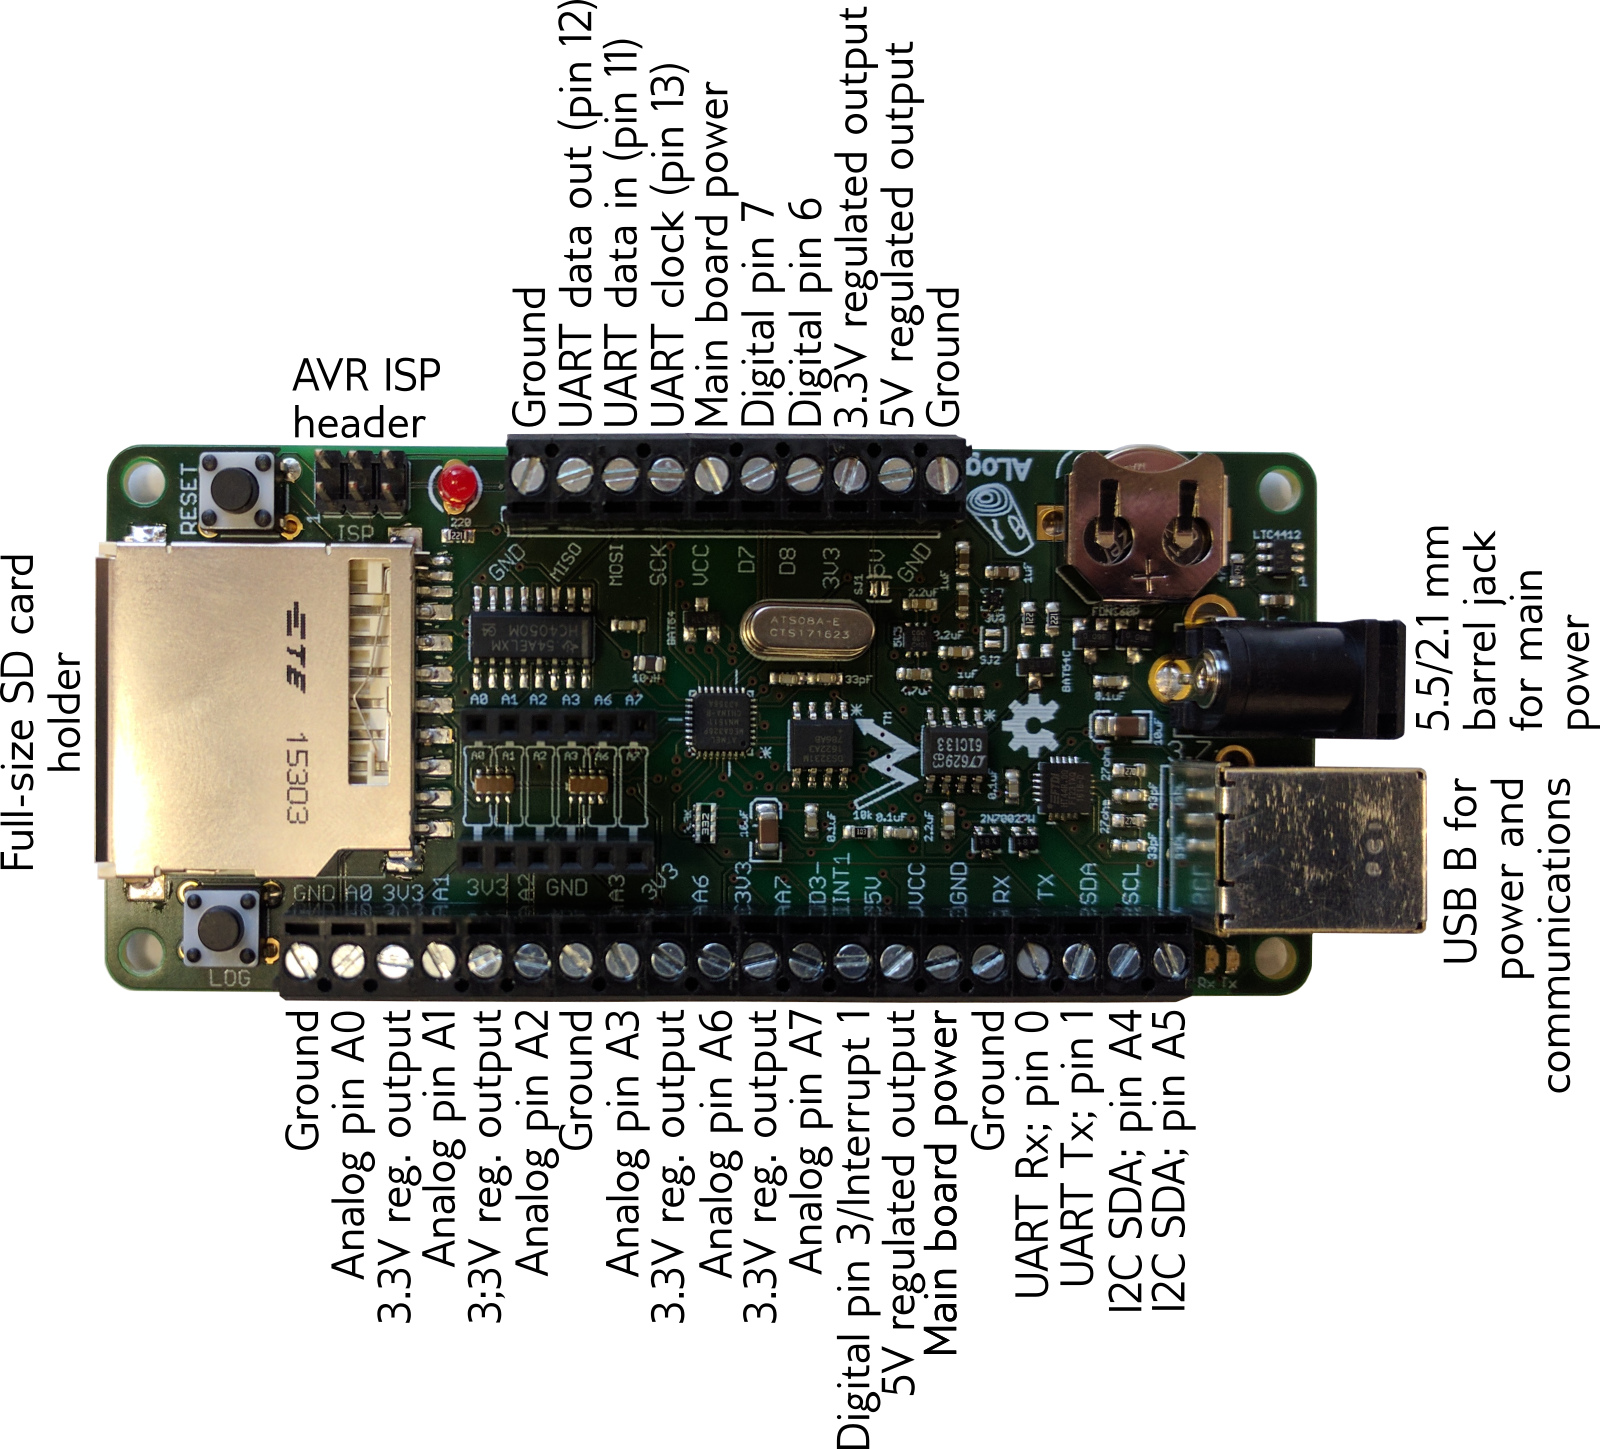
\includegraphics[width=\linewidth]{LoggerPinout.png}
\caption{A\+Log pinout and peripherals.}
\end{DoxyImage}


{\bfseries Notes} 
\begin{DoxyEnumerate}
\item All pin numbers correspond to those of the Arduino Uno
\item All S\+PI pins (11, 12, 13) are also used for SD card communication)
\item V\+CC means \char`\"{}\+Voltage of the Common Connector\char`\"{}
\item The 3.\+3V regulator is typically a precision voltage reference (part number L\+T1461\+D\+H\+S8-\/5\#\+P\+BF) that can source 10-\/50 mA of power, depending on V\+CC\+: 10 mA corresponds to 0.\+20V dropout between V\+CC and 3.\+3V; 50 mA corresponds to 1.\+5V dropout. Projects that need more power and/or use fully ratiometric measurements can request an A\+Log without this part; solder jumpers on the board will connect 3\+V3 pins to the unused side of our standard 3.\+3V low-\/dropout regulator.
\item The 5V regulated output is supplied via a charge pump; when no current is drawn, its voltage will increase to 5.\+2V; after some current draw, is output will drop to a stable 5V. If there is a concern about low voltage draw from the charge pump, users should monitor its voltage with a voltage divider connected to one of the analog channels, and include a reading during the time that the sensor or other load on the charge pump is on and active.
\item The interrupt pin (digital pin 3) can be used to detect events, such as an anemometer spinning or a rain gauge bucket tipping.
\end{DoxyEnumerate}\hypertarget{index_About}{}\section{About}\label{index_About}
Who is Northern Widget? What is the connection to the University of Minnesota?

{\bfseries Northern Widget} is a company that 